\documentclass[french, utf8]{article}
\usepackage[utf8]{inputenc}
\usepackage[T1]{fontenc}
\usepackage[french]{babel}
\usepackage[parfill]{parskip}
\usepackage{amsmath}
\usepackage{amssymb}
\usepackage{amsfonts}
\usepackage{graphicx}
\usepackage{subfigure}
\usepackage[font={small}]{caption}
\usepackage{float}
\usepackage{listingsutf8}
\usepackage{fullpage}
\usepackage[nochapter]{vhistory}
\usepackage{glossaries}
\usepackage{hyperref}
\usepackage{titlesec}
\usepackage{xcolor}



% -----------------------------------------------------
% -----------------------------------------------------
% -----------------------------------------------------

\makeglossaries

\newacronym{TLS}{TLS}{Transport Layer Security}

\hypersetup{
%couleurs des liens cliquable changée pour une meilleur lisibilité
    colorlinks=true,
    linkcolor=blue,
    filecolor=magenta,
    urlcolor=cyan,
    pdfpagemode=FullScreen,
    }

\title{INFO-F209 - Projet d'informatique 2 }
\author{Anton Romanova, Mohammad Secundar, Esteban Aguililla Klein, Vlad Moruntale, Mathieu Van Den Bremt, Nabil Abdellaoui, Ayman Boulaich, Noé Bourgeois}
\date{Novembre 2021}

\begin{document}
\maketitle
\tableofcontents
\newpage


% -----------------------------------------------------
% -----------------------------------------------------
% -----------------------------------------------------
\section{Introduction}
% -----------------------------------------------------
\subsection{But}
Faire un portage du jeux de plateau classique multijoueur Quoridor\footnote{les règles détailles peuvent être consultée dans la section \nameref{sec:Annexes}} par le biais d'une interface client-serveur et l'ajout de fonctionnalité sociale modernes.
\\ \\
Pour que la partie se termine, dans le mode classique, il suffit d'atteindre le côté opposé du plateau tout en empêchant l'adversaire de faire de même à l'aide de murs plaçables.    %TODO: dans le mode X, il faut Y
\\ \\
Concernant les fonctionnalités sociales, il est possible de gérer une liste d'amis, discuter avec ces derniers, créer une partie privées et consulter un classement des joueurs.
\\ \\
De par sa nature simple, le jeu se veut tout public malgré ses fonctionnalités sociales non modérées.  %ressemblance avec réseau social donc >13 ans min ???

% -----------------------------------------------------
\subsection{Glossaire}

\printglossary

% -----------------------------------------------------
% AJOUTEZ TOUS VOS CHANGEMENTS ICI
\subsection{Historique du document}

\begin{versionhistory}
\vhEntry{0.2}{24.11.21}{Bourgeois Noé }{Base De Données}
\vhEntry{0.2}{23.11.21}{Bourgeois Noé }{Logging}
\vhEntry{0.1.9}{21.11.21}{Romanova Anton, Ismaël Secundar}{Section ``Style de programmation’’ et ``Internationalisation et Localisation’’}
\vhEntry{0.1.9}{21.11.21}{Romanova Anton, Ismaël Secundar}{Ajout de la sous-section 3.2.3 (Concurrence)}
\vhEntry{0.1.8}{21.11.21}{Bourgeois Noé }{Actualisation du classement, colorisation du texte, hyperreferences, use case de gestion de compte}
\vhEntry{0.1.7}{20.11.21}{Bourgeois Noé }{Lancement, enregistrement, créer une partie, rejoindre une partie}
\vhEntry{0.1.6}{20.11.21}{Mathieu Van Den Bremt \& Nabil Abdellaoui}{Modification des UseCase et amélioration divers pour User requirements}
\vhEntry{0.1.9}{19.11.21}{Romanova Anton, Ismaël Secundar}{Brouillon pour besoins non-fonctionnels des besoins système}
\vhEntry{0.1.5}{19.11.21}{Aguililla Klein Esteban \& Moruntale Vlad}{Ajout du but et d'un annexe}
\vhEntry{0.1.4}{19.11.21}{Mathieu Van Den Bremt }{Tableau Use Case}
\vhEntry{0.1.3}{19.11.21}{Boulaich Ayman }{Sous section des besoins fonctionnels du système et début }
  \vhEntry{0.1.2}{18.11.21}{Anton Romanova}{Ajouts de la section "Annexes" et "Design"}
   \vhEntry{0.1.1}{17.11.21}{Mathieu Van Den Bremt \& Nabil Abdellaoui}{Début Besoin d'utilisateur + diagrammes Use Case}
  \vhEntry{0.1}{16.11.21}{Anton Romanova}{Structure générale}
\end{versionhistory}

% -----------------------------------------------------
% -----------------------------------------------------
% -----------------------------------------------------
\newpage
\section{Besoin d'utilisateur}
% -----------------------------------------------------

\subsection{Besoins/Exigences fonctionnelles}
%Connexion
%Démarrer une partie
%Actions durant une partie
%Visualisation classement
\subsubsection{Inscription et connexion}
L'utilisateur doit être capable de présenter un nom de compte ainsi qu'un mot de passe au démarrage du jeu pour pouvoir se connecter et accéder à son menu principal. Si il n'a pas de compte ou si il désire en recréer un, il lui est possible d'en créer un nouveau. Pour la création d'un compte, aucun mail n'est nécessaire à introduire, l'utilisateur doit juste présenter un nouveau pseudonyme accompagné d'un mot de passe pour terminer le processus de création. \newline


\begin{figure}[ht]
     \centering
    %\includegraphics[width=70mm,scale=0.1]{Image/SystemUC.PNG}
    \includegraphics[width=100mm,scale=0.1]{Image/ConnectionUC.PNG}

\end{figure}
\begin{center}
\begin{tabular}{|m{3cm}|m{3cm}|m{3cm}|m{3cm}|m{3cm}|}
\hline  Use Case & Pré condition      &  Post condition  & Cas général & Cas exceptionnels\\
\hline Register& l'utilisateur n'a pas  encore un compte & On enregistre le nouveau compte & Le programme demande un nom et un mot de passe & Si le nom est déjà utilisé alors on envoie une erreur  \\
\hline Connect  & L'utilisateur a déjà un compte & L'utilisateur rentre dans le programme & Le programme vérifie les informations donnée par le client ensuite, il lui permet de continuer sur le programme & Si les informations sont incorrects, alors on envoie une erreur \\
\hline Reset Password  & L'utilisateur a déjà un compte & Le mot de passe est modifié & Le programme demande à l'utilisateur de remplir les conditions d'un TOTP et/ou une question secrete, ensuite permet de modifié le mot de passe & Si l'utilisateur ne remplit pas les conditions alors on ne l'autorise pas à modifié son mot de passe \\
\hline
\end{tabular}\\
\end{center}
\subsubsection{Écran Principal}
\label{sec:MenuPrincipalUser}
Après connexion, l'utilisateur aura accès à différentes fonctionnalités. Tout d'abord, une multitude d'interactions utilisant un réseau lui sera disponible. Il pourra gérer une liste d'amis et/ou discuter avec eux en s'échangeant des messages, il pourra aussi accéder à un  classement des meilleurs joueurs. Et c'est bien à partir du menu que l'utilisateur pourra créer et lancer une partie. \newline


L'utilisateur pourra configurer sa partie en modifiant plusieurs paramètres. Il devra indiquer le nombre de participants qui seront de la partie, ils pourront être 2 à 4. Par la suite, il devra indiquer quels joueurs, parmi la liste d'amis, rejoindront la partie. Les joueurs invités devront évidemment confirmer leur participation. Une fois tout ceci fait, les joueurs rejoindront automatiquement un unique salon et seront tous redirigés vers la partie nouvellement lancée. \newline

Si le cours d'une partie a été précédemment sauvegardé, l'utilisateur pourra la reprendre là où elle s'était arrêté à condition que tout les autres participants soient présents pour continuer.

Si il le désire, l'utilisateur pourra aussi demander de l'aide, l'application affichera le fonctionnement du jeu et les différentes fonctionnalités de cette dernière.

%\newline

\begin{figure}[ht]
     \centering
    %\includegraphics[width=70mm,scale=0.1]{Image/SystemUC.PNG}
    \includegraphics[width=150mm,scale=0.1]{Image/MainScreenUC.png}

\end{figure}


\begin{center}
\begin{tabular}{|m{3cm}|m{3cm}|m{3cm}|m{3cm}|m{3cm}|}
\hline  Use Case & Pré condition      &  Post condition  & Cas général & Cas exceptionnels\\
\hline Check Ranking & Un classement existe  & L'utilisateur voit le classement & Le programme montre le classement des joueurs & Néant \\
\hline Manage friend list & Néant & La list est modifiée si l'utilisateur le veut & Le programme ouvre la liste d'amis & Néant \\
\hline Send Message & Utilisateur cible existe & Le message est envoyé & Le programme envoie un message écrit par l'utilisateur à une personne de la liste d'amis de celui-ci & Néant \\
\hline Add Friend & L'ami qui doit être ajouter à la liste existe & La liste est modifiée & Le programme sauvegarde le contact du nouvel ami dans la liste & Si le nouvel ami n'existe pas  alors on envoie une erreur à l'utilisateur \\
\hline Delete Friend & L'ami qui doit être supprimé de la liste ést dans la liste & La liste est modifiée & Le programme supprime le contact de l'ami dans la liste & Si l'ami n'est pas dans la liste alors on envoie une erreur à l'utilisateur \\
\hline Create Game & Néant & Néant & Le programme lance la configuration d'une partie puis lance celle ci après avoir lancer l'invitation d'un joueur & Néant \\
\hline Configure Game & Une partie est sur le point d'être créée  & Les paramètres de la partie change & Le programme permet à l'utilisateur de choisir les paramètres de sa partie & Néant \\
\hline Invite Friend to Game & L'ami invité doit faire partie de la liste d'ami & L'ami rejoinds la partie & Le programme permet à l'utilisateur d'inviter un ami à jouer avec lui & Si l'ami refuse l'invitation, le programme demande à l'utilisateur d'inviter un autre ami \\
\hline Join Game by invitation & Un autre utilisateur a invité l'utilisateur & L'utilisateur rejoinds la partie & Le programme invite l'utilisateur à rejoindre une partie & Si l'utilisateur refuse alors le programme envoie un message à l'utilisateur ayant envoyé l'invitation \\
\hline Joined Saved Game & Une partie sauvegardée existe et l'utilisateur qui a joué précédement accepte de jouer & La partie sauvegardée est lancée & Le programme reprends la partie sauvegardée  & Si l'autre utilisateur refuse ou si la partie sauvegardée n'existe pas ou ne peut être lancée, le programme renvoie une erreur \\
\hline
\end{tabular}\\
\end{center}

\newpage
\begin{center}
\begin{tabular}{|m{3cm}|m{3cm}|m{3cm}|m{3cm}|m{3cm}|}

\hline Play Game & Néant & En fin de partie les résultat sont mis à jour dans le classement & Le programme démarre la partie & Si la partie est quittée en cours de jeu, alors le classement n'est pas mis à jour \\
\hline Get Help & Néant & Néant & Le programme affiche l'aide pour le programme et les règles du jeu & Néant \\
\hline Disconnect  & Néant & Le programme retourne à l'écran de connexion & Le programme déconnect le joueur & Néant \\
\hline Delete account  & Néant & L'utilisateur est déconnecté et son compte est supprimé & Le programme supprime le compte & Néant \\
\hline
\end{tabular}\\
\end{center}

\subsubsection{Durant une partie}
Quand c'est son tour, le joueur doit pouvoir effectuer une action, déplacer un pion ou mettre un mur. Cette action est représenté comme un message envoyé à l'application qui agira sur lui même en conséquence.
En plein duel, l'un des joueurs peut proposer au reste des participants de mettre le jeu en pause et de sauvegarder la partie en cours pour pouvoir la continuer plus tard. Les joueurs peuvent aussi déclarer forfait et donc se retirer.
Si l'un des joueurs se déconnecte sans proposer de sauvegarder la partie, il est considéré comme disqualifié, ses murs posés seront toujours présents mais ses pions se retrouveront retirés du plateau.
\newline

\begin{figure}[ht]
     \centering
    %\includegraphics[width=70mm,scale=0.1]{Image/GameUC.PNG}
    \includegraphics[width=110mm,scale=0.1]{Image/GameUC.png}

\end{figure}
%ligne vide tableau : \hline .  & . & . & . &. \\
\begin{center}
\begin{tabular}{|m{3cm}|m{3cm}|m{3cm}|m{3cm}|m{3cm}|}
\hline  Use Case & Pré condition      &  Post condition  & Cas général & Cas exceptionnels\\
\hline Play Game& L'utilisateur à lancer et configurer une partie et il y a un nombre requis de Joueur & A la fin de la partie on retourne sur l'écran principal & Le programme lance le jeu Quoridor et demande tour par tour, quel actions les joueur veulent faire & Si un joueur quitte en cours de partie un message est envoyé à l'adversaire  \\
\hline Move pawn  & Le pion peut être déplacer comme le veut l'utilisateur & Le plateau est modifié avec la nouvelle position du pion & Le programme déplace le pion & Néant \\
\hline Place Wall  & L'emplacement désigné pour le mur est libre et ne bloque pas entièrement un pion & Le plateau est modifié avec le nouveau mur & Le programme place un mur dans la position choisie & Néant \\
\hline Pause Game  & Néant & Le jeu est mis en pause, sauvegardé et ensuite terminé & Le programme demande à l'adversaire si celui-ci accepte de mettre en pause le jeu & Néant \\
\hline Save  & Le jeu a été mis en pause sur l'accord des deux joueurs & La partie est sauvegardée & Le programme sauvegarde la partie tel qu'elle est & Si le programme n'a pas réussi à sauvegarder les données, alors celui-ci envoie un message d'erreur \\
\hline Forfeit  & Néant & La partie est terminée sur une victoire adverse & Le programme termine la partie & Néant \\
\hline
\end{tabular}\\
\end{center}

% -----------------------------------------------------
\newpage
\subsection{Exigences non-fonctionnelles}
\subsubsection{Compte}
\textcolor
Le programme doit vérifier si le compte présenté au démarrage de l'application existe. Si le pseudonyme inséré n'est pas valide ou si le mot de passe n'est pas le bon, l'application empêche tout accès au menu principal.
\newline

%L'utilisateur pourra

%\\
L'utilisateur peut néanmoins en créer un nouveau. Si, lors d'un enregistrement, un nouveau pseudonyme est entré et n'est pas reconnu par l'application depuis sa base de donnée, celui-ci pourra être utilisé pour créer un nouveau compte, l'application agit ainsi pour ne pas créer de doublons.
\newline
\subsubsection{Interface}
La version simpliste de ce programme affiche un plateau de jeu en deux dimensions dans un terminal de commande et propose des modèles et des couleurs assez limités. \newline
Par après, une version beaucoup plus performante et présentable sera affiché grâce à une interface graphique.
\subsubsection{Latence}
Toutes les actions doivent passer d’un utilisateur à un autre avec une latence minimale en mettant à jour le plateau le plus rapidement possible et ainsi donner l'illusion que les actions se font instantanément.
\subsection{Légalité}
L'utilisateur doit pouvoir supprimé son compte selon le GDPR.
\subsubsection{Messagerie}
L'utilisateur pourra voir la date et l'heure d'envoie d'un message.
\subsubsection{Déconnexion en partie}
Dans le cas d'une deconnexion durant une partie, soit la partie s'arretera si il n'y que 2 joueur, soit le joueur restant de l'équipe devra jouer avec le pion n'ayant plus de joueur.

% -----------------------------------------------------
% -----------------------------------------------------
% -----------------------------------------------------
\section{Besoins du système}

% -----------------------------------------------------
\subsection{Besoins fonctionnels}
\\\nameref{sec:Lancement}
\\\nameref{sec:Enregistrement}
\\\nameref{sec:Connexion}
\\\nameref{sec:MenuPrincipalSystem}
\\\nameref{sec:GestionDeCompte}
\\\nameref{sec:CréationDePartie}
\\\nameref{sec:GestionDePartie}
\\\nameref{sec:ActualisationDuClassement}
\\\nameref{sec:BaseDeDonnées}
\\\nameref{sec:Logging}
\\\nameref{sec:Server}


\subsubsection{Lancement}
\label{sec:Lancement}
Le programme, à son lancement,
affiche une fenêtre d'accueil contenant le titre du jeu et demande à l’utilisateur d'entrer
\\un pseudo et
\\un mot de passe.

%Il peut ensuite
%\\soit créer un nouveau compte,
%\\soit se connecter avec un compte déjà %enregistré dans une base de
%donnée.

\subsubsection{Enregistrement}
\label{sec:Enregistrement}

%TOTP?
Conditions:
\item- Le pseudo n'est pas présent dans la Base De Donnée et contient:
\item--- uniquement des caractères alphanumériques + "$_$" + "-"
\item--- un nombre de caractères entre 3 et 25

\item- Le mot de passe contient:
\item--- plus de 8 caractères
\item--- 4 caractères spéciaux

Si les conditions sont respectées, le programme
demande à l'utilisateur une réponse à une question secrète puis de confirmer la création d'un
nouveau compte.
\\Si l'utilisateur confirme, le compte, le mot de passe et la question secrète sont enregistrés dans
la base de données et la fenêtre du
\nameref{sec:MenuPrincipalSystem}
 apparaît.

\subsubsection{Connexion}
\label{sec:Connexion}
Lorsque l'utilisateur lance le programme il devra se connecter via un nom d'utilisateur et un mot de passe s'il  possède un compte.
Si l'utilisateur ne possède pas de compte il aura la possibilité de s'enregistrer et ainsi de faire en sorte que son compte soit stocké dans la base de données.
%---------------------------------------------
\newline
\\Si l’utilisateur demande à se connecter,
        \\Si le pseudo se trouve dans la base de donnée,
            \\et le mot de passe correspond,
                \\le programme établit la connexion entre l'utilisateur et le serveur
                puis affiche le menu principal.
        \\Si le pseudo ne se trouve pas dans la base de données,
            \\il avertit l'utilisateur que ce compte n'est pas enregistré.
        \\Si le pseudo s'y trouve, mais le mot de passe ne correspond
pas,
            il avertit l'utilisateur en conséquence.
\newline

\newline
%-------------------------------------------
use case
supp compte
Question: quelle moyen utilisé pour retrouver son compte avec mot de passe oublié ? question personnelle
\subsubsection{Menu principal}
\label{sec:MenuPrincipalSystem}

Use case: \nameref{sec:MenuPrincipalUser}


\subsubsection{Gestion du compte}
\label{sec:GestionDeCompte}
L'utilisateur pourra modifier son compte lorsqu'il est connecté via ce dernier au programme.L'utilisateur aura plusieurs possibilités lors de la modification de son compte tels que changer sa photo de profil , son nom d'utilisateur, son mot de passe , ajouter une description . Les modifications réalisées par l'utilisateur seront sauvegardées dans la base de données .
%Description dans le use case
\begin{figure}[ht]
     \centering
    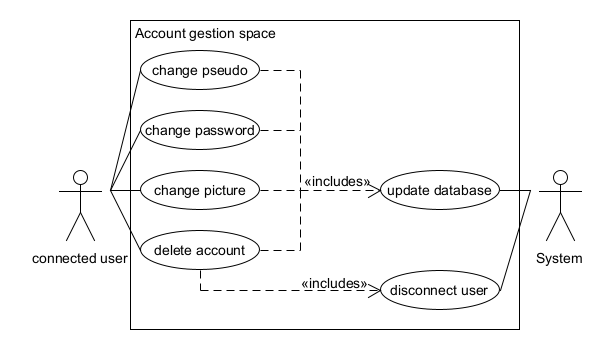
\includegraphics[width=110mm,scale=0.1]{Image/AccountGestionUC.png}
\end{figure}

\begin{center}
\begin{tabular}{|m{3cm}|m{3cm}|m{3cm}|m{3cm}|m{3cm}|}
\hline  Use Case & Pré condition      &  Post condition  & Cas général & Cas exceptionnels\\

\hline Change Pseudo  & conditions d'\nameref{sec:Enregistrement} du pseudo & Le nouveau pseudo est affiché à la place de l'ancien, le nombre de comptes dans la BDD n'a pas changé & Le programme remplace dans la BDD l'ancien pseudo par le nouveau & Néant \\
\hline Change Password  & conditions d'\nameref{sec:Enregistrement} du mot de passe & L'ancien mot de passe n'est plus valide & Le programme remplace dans la BDD l'ancien mot de passe par le nouveau & Néant \\
\hline Change picture  & L'image est d'un format compatible JPEG ou PNG et n'est pas corrompue & La nouvelle photo est affichée à côté du pseudo de l'utilisateur & Le programme remplace dans la BDD l'ancienne image par la nouvelle & Si l'image est d'une définition supérieure au maximum fixé, celle-ci est compressée \\
\hline Delete Account  & Néant &  Le programme déconnecte l'utilisateur  & Le programme supprime dans la BDD toutes les données liées au pseudo du joueur & Néant \\
\hline
\end{tabular}\\
\end{center}


\subsubsection{Configuration de partie}
\paragraph{Création de partie}
\label{sec:CréationDePartie}
Si l’utilisateur sélectionne
"new game",
une fenêtre de configuration de jeu apparaît contenant les paramètres par défaut: \\
    -la taille du plateau sous forme d'un nombre\\
    %-le nombre de pions\\
    -l'apparition aléatoire de murs sur le plateau sous forme de switch\\
    -le ou les autre(s) joueur(s):
\item---  une ou des IA(s) et sa/leur(s) difficulté(s)
\item---  un ou des humain(s) qui ont rejoint sous forme de tableau.
    -l'invitation d'autres joueurs humains sous forme de bouton à cliquer pour ouvrir une fenêtre affichant les joueur connectés et un espace de recherche
\\L'utilisateur peut les modifier et, à tout moment, démarrer la partie avec les paramètres
affichés

\paragraph{Rejoindre une partie}
\\Si l’utilisateur sélectionne
"join", une liste des joueurs créant une partie apparaît.
\\Il peut en sélectionner une pour la rejoindre.
\\Si l’utilisateur reçoit une invitation, celle-ci est affichée superposée à la fenêtre actuellement affichée sauf si il est en train de jouer.

\subsubsection{Gestion de partie}
\label{sec:GestionDePartie}
%#TODO
Lorsque le joueur lance la partie le plateau du jeu s'affiche en fonction des options de jeu choisi par les joueurs.le système gère alors les différentes manipulation que peut faire les joueurs. le joueur peut mettre pause au jeu et déclarer forfait via des boutons sur les cotés  . le système doit aussi actualiser le plateau lorsque le joueur bouge ou place un mur. le nombre de murs de chaque joueur est connue par le système et est décrémenté à chaque fois que le joueur place un mur sur le terrain.


\subsubsection{Actualisation du classement}
\label{sec:ActualisationDuClassement}

Après la partie, le classement est mis à jour:
\\-Si c'est une égalité, les scores ne changent pas.
\\-Si le classement du gagnant était plus bas,
son classement devient celui du perdant avant d'être augmenté

les classements des gagnant et perdant sont respectivement augmenté et diminué de \\
\[
 \text{(taille du plateau + le nombre de murs)} \mod \text{nombre de tours}
\]

\subsubsection{Base de données}
\label{sec:BaseDeDonnées}

La base de donnée \href{https://en.wikipedia.org/wiki/SQL}{SQL} contient :
\item- les données correspondant à chaque joueur:
\item--- pseudo (:clé)
\item--- mot de passe % Salted hash + salt
\item--- chemin d'accès vers le fichier de l'image de profil
\item--- classement
\item--- liste d'amis
\item--- liste de conversations
\item--- liste de parties enregistrées

\item--- les conversations
\item- les parties enregistrées
%\\ \item--- la liste des participants
\item- le classement

\subsubsection{Logging}
\label{sec:Logging}
Tout événement du programme incluant un accès à la BDD est enregistré sous forme ASCII ou binaire dans un log file et consultable par l'administrateur système sous forme ASCII.

\colorbox{red}{\subsection{Serveur->Design ?}
\label{sec:Server}}



% -----------------------------------------------------
\subsection{Besoins non-fonctionnels}
Contraintes liées au matériel

\subsubsection{Portabilité}

Le programme doit fonctionner sur Linux. Si possible sans trop de modifications, il devrait également être compatible avec Windows.

\subsubsection{Réseau}

Les clients et le serveur doivent être connectés à un même réseau. Lorsqu'un joueur se déconnecte subitement du serveur, le serveur doit en avertir d'autres serveurs clients qui ont une partie en cours avec le joueur déconnecté.

\subsubsection{Concurrence}

Afin de pouvoir gérer plusieurs connections, le programme serveur doit s'exécuter en parallèle. Les transactions de la base de données effectuées en concurrence ne peuvent pas violer l'intégrité des données. Le contrôle optimiste de la concurrence sera utilisé, pour améliorer les performances et éviter les deadlocks.

Du côté client, la concurrence doit également être utilisée pour avoir une interface graphique utilisateur (GUI) réactive.

\subsubsection{Sécurité}

Pour que l'envoi de données sensibles à travers internet ne puisse pas être intercepté, la communication devra se faire à l'aide d'un protocole de communication crypté. Un choix évident serait le \acrfull{TLS}.

Une session pourra rester active à l'aide d'un access token.
Ce token aura une date d'expiration. Le programme client gardera ce token dans la RAM.
Ainsi, après le redémarrage du programme client, l'utilisateur devra se reconnecter avec son nom d'utilisateur et son mot de passe.


En ce qui concerne le programme serveur, celui-ci gardera un salted hash du mot de passe dans la base de données.

La récupération de mots de passes pourra se faire avec des questions secrètes ou éventuellement avec des mots de passes à usage unique générés à l'aide du standard TOTP (le client pourra, par exemple, les générer avec Google Authenticator ou l'altérnative open-source, RavioOTP).

\subsubsection{Fiabilité}

Load balancer, horizontal scaling, ... Then deployment diagram?

Lorsque le client se déconnecte du serveur au cours d'une partie, l'adversaire doit en être averti.
Après une minute d'attente, le joueur déconnecté est déclaré perdant suite à un abandon.

\subsubsection{Internationalisation et Localisation}

Dans le contexte de ce projet d'année, le programme ne sera pas internationalisé.
Les timestamps (date des messages, création de parties, ... ) seront enregistrés en timestamp unix. Ainsi, les clients se trouvant dans un fuseau horaire différent pourront voir ces timestamps en heure locale

\subsubsection{Possibilité d'évolution}


\subsubsection{Légalité}


Do we actually need GDPR complience?
Ce programme n'aura pas de politique de confidentialité.
Suite à une demande de la part de l'utilisateur, tout le contenu de son compte sera supprimé.

% -----------------------------------------------------
\subsection{Exigences du domaine}

% -----------------------------------------------------
% -----------------------------------------------------
% -----------------------------------------------------

\section{Design et fonctionnement du sytème}
\colorbox{green}{\subsection{Serveur ?}
\label{sec:Server}}

% -----------------------------------------------------
% -----------------------------------------------------
% -----------------------------------------------------

\newpage
\section{Annexes}
\appendix

\label{sec:Annexes}
\section{Style de programmation}

Dans le cadre de ce projet, le style de programmation défini par Google:
\\ \href{https://google.github.io/styleguide/cppguide.html}{https://google.github.io/styleguide/cppguide.html}
\\ see \href{https://google.github.io/styleguide/cppguide.html#Naming}{Google Naming conventions}
\\doit être utilisé.

En résumé,
\begin{itemize}
	\item L'indentation est de 2 espaces,
	\item Les noms de fichiers en minuscules avec des ``-’’ et des ``\_’’
	\item Les noms de classes, des structs et des méthodes sont en CamelCase et commencent par une majuscule
	\item Les noms de variables sont en minuscules et séparés par des ``\_’’
	\item Les attributs privés terminent par un ``\_’’
	\item les constantes sont en CamelCase et commencent par un k minuscule (ex: kRefreshRate)
\end{itemize}

\section{Règles de base de Quoridor}
Ces dernières peuvent être consultées sur le site de son éditeur Gigamic \href{https://www.gigamic.com/files/catalog/products/rules/quoridor-classic-fr.pdf}{https://www.gigamic.com/files/catalog/products/rules/quoridor-classic-fr.pdf}


\end{document}
